\documentclass[accentcolor=tud0b,12pt,paper=a4]{tudreport}

\usepackage[utf8]{inputenc}
\usepackage{ngerman}
\usepackage{parcolumns}

\newcommand{\titlerow}[2]{
	\begin{parcolumns}[colwidths={1=.15\linewidth}]{2}
		\colchunk[1]{#1:} 
		\colchunk[2]{#2}
	\end{parcolumns}
	\vspace{0.2cm}
}

\title{Open Diabetes UAM Heuristik Algorithm}
\subtitle{Pflichtenheft UAM}
\subsubtitle{%
	\titlerow{Gruppe 11}{%
		Aino Schwarte <aino.schwarte@stud.tu-darmstadt.de>\\
		Anna Mees <anna.mees@stud.tu-darmstadt.de>\\
		Jan Paul Petto <janpaul.petto@stud.tu-darmstadt.de>\\
		Paul Wolfart <paul.wolfart@stud.tu-darmstadt.de>\\
		Tom Großmann <tom.grossmann@stud.tu-darmstadt.de>}
	\titlerow{Teamleiter}{Benedikt Schneider <schneider-benedikt@gmx.net>}
	\titlerow{Auftraggeber}{%
		M.Sc. Jens Heuschkel <heuschkel@tk.tu-darmstadt.de>\\
		Telecooperation\\
		Smart Urban Networks}
	\titlerow{Abgabedatum}{01.12.2018}
\institution{Bachelor-Praktikum WS 2018/2019\\Fachbereich Informatik}}

\begin{document}

	\maketitle
	\tableofcontents 
	\newpage
	\chapter{Zielbestimmnung}
	
	Das Projekt Open Diabetes UAM Heuristik Algorithmen entwickelt ein Programm zur richtigen Erkennung von Mahlzeiten anhand der Blutwerte die ein Sensor bei Insulinpatienten misst. Anhand dieser Daten soll die Höhe und der richtige Zeitpunkt für die nächste Insulindosis bestimmt werden. Nightscout stellt dabei eine Onlineplattform zur grafischen Darstellung der Werte dar. 
	\section{Analyse}

Für das Projekt stehen folgende Infrastrukturen zur Verfügung: 
\begin{itemize}
	\item Anonymisierte Patientendaten zum Testen der Ansätze
	\item Nightscout um eigene Instanzen aufzusetzen 
	\item Beschreibungen der Tools
	\item Paper mit Ansätzen zur Berechnung der Insulin- und Kohlenhydratwerte
\end{itemize}
	
	\section{Soll Analyse}

Folgende Punkte müssen implementiert bzw. erstellt werden:

\begin{itemize}
	\item Skript das die Daten aus den Nightscout Instanzen ausliest und wieder zurück schreibt
	\item Parser der den Datensatz und die Daten aus dem Skript in Java überführt
	\item Wikiartikel wie die Daten aus Nightscout auf unsere Daten abgebildet werden
	\item Kommandozeilentool zum Lesen, Schreiben und Synchronisieren von Nightscout
	\item Wikiartikel mit einer Anleitung für das Kommandozeilentool
	\item Berechnung von:
	\begin{itemize}
		\item Insulin on board
		\item Carbs on board
		\item Basalwerte
	\end{itemize}
	\item Wikiartikel der die Algorithmen und mögliche Einstellungsfaktoren beschreibt
	\item Plotten der Daten
	\item Modifikation von Nightscout um berechnete Kohlenhydrate getrennt von tatsächlichen darstellen zu können.
\end{itemize}
	
	\section{Anforderungen}
	\subsection{funktional}
\begin{itemize}
	\item Das Programm muss Mahlzeiten korrekt platzieren um den Insulinspiegel konstant zu halten
	\item  
\end{itemize}
	
	\subsection{nicht-funktional}
\begin{itemize}
	\item Das Programm muss auf einem PI Zero in angemessener Zeit laufen
\end{itemize}
	
	\chapter{Grobarchitektur}
	
	\centering
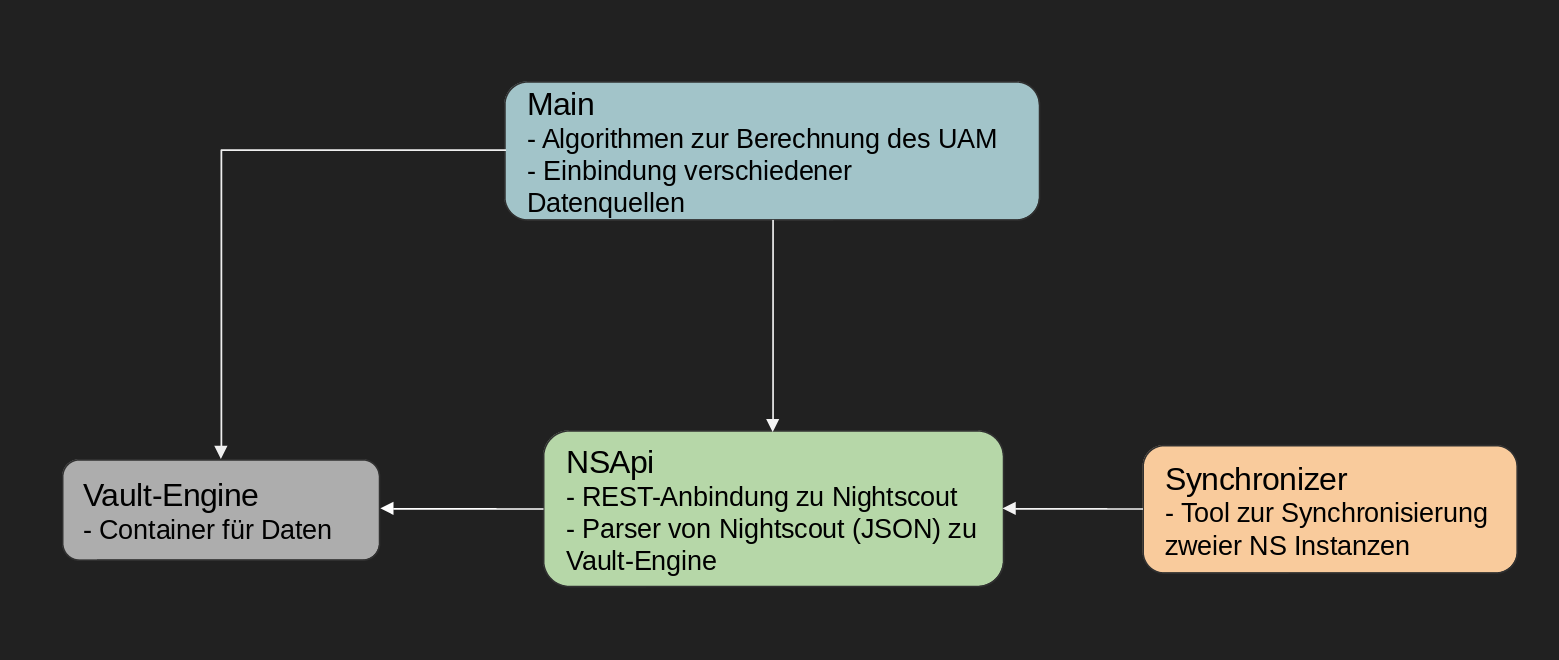
\includegraphics[width=0.7\textwidth]{architektur.png}
	
	\section{Qualitätssicherung}
	Siehe QS-Dokument.
	
	\section{Risikomanagement}
	
	\section{Rechtliches}
	
	Wir entwickeln unter der AGPLv3-Lizenz und verwenden nur Open-Source Quellen. Dadurch vermeiden wir Copy-Right-Verletzungen und schließen jede Garantie an unserem Code aus.
	
\end{document}
